\setcounter{chapter}{1} 
\chapter{Theoretical Background/ Climate and Cloud Physcis} \label{ch:theoretical_back}
This chapter describes the necessary theoretical background on clouds for this study. It is organised as follows. The three first sections describe the cloud's role in both present and future climate systems. Beginning with cloud formation and dissipation, including the cloud effects on Earth's radiative budget in the current climate and the suggestion of future cloud climatologies as proposed by \acrshort{ipcc} in \acrshort{ar5}. This is followed by a brief introduction to parameterization of clouds, i.e. the method used to incorporate clouds into climate models.
% Therefore necessary in studies of cloud feedback's. %in future climates. 
Finally, the data used in the compilation of the \acrshort{ecc} dataset is introduced. 

\section{Clouds role in the climate system} \label{sec:cloud_in_climate_system}
% Clouds, climate and machine learning
Clouds play an important role in the climate system both affecting the radiative budget and the hydrological cycle. Understanding how clouds form in the complex system of the atmosphere involves both knowledge about the large scale influence by the circulation and the small scale influence by aerosols. Clouds exist in countless number of shapes and sizes, and have fascinated mankind since the beginning of time. Figure \ref{fig:cloud_cover_jotunheimen} shows the stunning view from Store Smørstabbtinden in Jotunheimen. The sky is covered by cumulus type clouds, a common sight in summer.
\begin{figure}
    \centering
    \adjincludegraphics[scale=0.1, trim={0 {.3\height} 0 0}, clip]{Chapter1_Intro/images/cloud_cover_ina.jpg}
    \caption[Cumulus deck at Store Smørstabbtinden in Jotunheimen]{Cumulus deck at Store Smørstabbtinden in Jotunheimen, photo by Ina Storteig.}
    \label{fig:cloud_cover_jotunheimen}
\end{figure}
%Climate models are the most useful tool for studying the past, present and future climate. Clouds and aerosols are acknowledged as the factors contributing with the largest uncertainty to the \acrfull{ecs}. Also known as global mean temperature increase as a consequence of doubling of the pre-industrial levels of $CO_2$ (280 \acrshort{ppm}). \textbf{kilde AR4 which ch?} \textit{It remains unclear to which level of sophistication is adequate to model their effect om climate.} (\cite{IPCC_CH7_clouds}).
%\newpage

\subsection{Evolution of clouds}
Clouds are composed of liquid droplets, ice crystal or both. To this day the microphysics of all phases are not fully understood \textcolor{red}{\textbf{kilde - les å sjekk at den kan brukes} \cite{ReviewMicroPhys}}. Here mixed phase clouds, consisting of both liquid and ice, have proven to be the most difficult to fully understand. 

\textit{Aerosols} include both liquid and solid particles suspended in the air. They interact with the clouds by serving as particles which vapour and ice can condensate or deposit upon. The different phases require different properties and the nuclei are called \acrfull{ccn} for liquid droplets and \acrfull{inp} for ice crystals. 
% Chemistry definition of saturation - the degree or extent to which something is dissolved or absorbed compared with the maximum possible, usually expressed as a percentage.
In the following discussion, \textit{saturation} describes the equilibrium state between to phases. % \textcolor{red}{er dette en definisjon du selv har funnet på? Eller har det fra et sted? }. 
For phases such as liquid water and vapour, saturation implies equal rates of condensation and evaporation. Phase changes occur when the system deviates from the equilibrium state. Under supersaturated conditions, the rate of condensation exceeds the rate of evaporation, facilitating vapour to condense onto suitable aerosols and initiating the formation of clouds. 
% The energy barrier needed to overcome (surface tension) to homogeneous nucleation 

Saturation is usually achieved by a temperature decrease in rising air masses. The saturation vapour pressure, $e_s$, is the quantity describing the maximum amount of vapour air can retain at a certain temperature. The way in which $e_s$ depends on the temperature, $T$, is described by the Clausius-Clapeyron equation for water, see Equation \eqref{eq:clausius_clapeyron_differentias}. The entalphy of vaporization, $l_v$, is the amount of energy needed to evaporate one unit (e.g one mole) of molecules from the liquid. This is also known as the latent heat of vaporization. 
\begin{equation} \label{eq:clausius_clapeyron_differentias}
    \frac{de_s}{dT} = \frac{l_v e_s}{R T^2}
\end{equation}
Here $l_v = 40.8 \cdot 10^3 J mol^{-1}$ and the universal gas constant $R= 8.314 J mol^{-1} K^{-1}$ (\cite{cloud_phys_book_johanne}, p. 42). 

A solution to Equation \eqref{eq:clausius_clapeyron_differentias} is given in Equation \eqref{eq:clausius_clapeyron}. It is derived by integrating from $T_0 = 273.15K \left(0 ^{\circ}C \right)$ to an arbitrary temperature, $T$. The integral is intractable for varying $l_v$. However a constant $l_v$ is %in most cases 
a reasonable assumption for the ranges of temperatures of atmospheric interest. The lower boundary, $T_0$, is chosen based on convenience, motivated by the fact that the constant of integration,  $e_0$, needs to originate from measurements. At $T_0$, the equilibrium of a mixture of water and ice at a total pressure of $1$ $atm$ is $e_0 = 611Pa$. 
\begin{equation} \label{eq:clausius_clapeyron}
    e_s\left( T \right) = e_0 e^{\frac{l_v}{R} \left( \frac{1}{T_0} - \frac{1}{T} \right) }
\end{equation}
From Equation \eqref{eq:clausius_clapeyron} it is clear that $e_s$ increases with rising temperature, resulting in the phenomena that warmer air can retain more vapour. The same principles apply for the phase change sublimation, but its entalphy, $l_s$, has a distinct value (\cite{cloud_phys_book_johanne}, p.135). The saturation vapour pressure with respect to ice, $e_i$, can be derived by replacing $l_v$ by $l_s$. Subsaturated conditions cause the cloud liquid water to evaporate, and ultimately the cloud disappears. This can happen when the cloud mixes with dry air or the temperature increase. The reverse process of adiabatic cooling, caused by sinking air masses in cloud. 

%From Equation \eqref{eq:clausius_clapeyron} it becomes clear that the  is inversely proportional with the second power of the temperature, meaning that for decreasing temperatures the vapour pressure 
%Double check if this id only valid for adiabatic processes, is there any other assumptions..?
%$R^*$ is the specific gas constant (the universal
%gas constant divided by the mean atmospheric molecular
%weight).  
Growth processes are phase dependent. Liquid droplets grow by diffusion and later by collision and coalescence. At temperatures around -38 $^oC$ (\cite{lohmann2016}, \textbf{p.222}, men det referes til pruppacher og klett 1997) droplets spontaneously freeze, while at warmer temperatures freezing can only occur with the aid of an  \acrshort{inp}. Clouds consisting purely of ice crystals first grow by deposition of vapour and then by aggregation (\cite{Fowler1996LiquidAssumptions}). In the presence of both phases, the Wegeron-Bergeron-Findeisen process describes the mechanism where droplets evaporate and the vapour deposits on to the ice crystals. %When both phases are present in a cloud, the saturation vapour pressure over ice is higher than over liquid. This may cause the droplets to evaporate and deposit on to the ice crystals. 
This mechanism exists because the saturation vapour pressure is lower with respect to ice than water, $e_i < e_s$. The process is most efficient at -12$^{\circ}C$ when the difference is largest.

%\section{Clouds role in the energy budget}

\subsection{Clouds role in the radiative budget}
\textbf{MOVE TO THE MOST SUITABLE SPOT. Macrophysical properties describe the clouds as units, using properties like base height, top height, thickness, fractional cover and regime (also known as type). Microphysical processes are all mechanisms involving the particles forming a cloud. Examples of properties used to quantify the microphysical state
are \acrshort{ccn} and droplet number concentrations (\cite{Grabowski2019ModelingBetter}).}
The characteristic white colour of the clouds has it nature in its ability to  effectively scatter solar radiation. %(explains why they appear white - because the backscatter radiation of all wavelenght in the visible spectrum)
%In part, this mechanism describes the important role in the Earth radiative budget. 
The Earth bathes in radiation from the Sun. Passing through the atmosphere, a small portion of the radiation gets absorbed while another portion gets scattered by clouds and aerosols. The majority of the radiation reaches the Earth and transforms into heat, warming the surface. The Earth emits thermal radiation, a minor portion of which escapes directly back to space, while most of it gets absorbed by the atmosphere and is re-emitted. This phenomena is known as \textit{the greenhouse effect}. 

The amount of heat trapped in the Earth system depends fundamentally on the spectral properties of its components (i.e. clouds, greenhouse gases, aerosols), and determines the magnitude of the enhanced warming (\cite{greenhouse_effect}).

%The physical properties of the atmospheric components determine their interactions with radiation. 
\textit{Albedo} is the ratio of reflected to incoming radiation. Dense low level clouds have high number concentrations of droplet, which corresponds to a large surface area. This results in enhanced scattering of radiation and thus a higher albedo. The greenhouse effect of clouds follows the principals of the greenhouse effect described above. It arises from their ability to absorb thermal radiation and re-emit it. The absorbed radiation originates from the surface or the atmosphere below. A widely used assumption is that the Earth (and most clouds) radiate like a black body, thus its radiant flux is given by Stefan-Boltzmann fourth-power law, 
\begin{equation} \label{eq:stefan-boltzmann}
    F = \sigma T ^4 % \epsilon
\end{equation}
here $F$ denotes flux in units of $W m^{-2}$, $T$ denotes temperature in units of $K$ and \\  $\sigma = 5.670 \time 10^{-8} W m^{-2} K^{-4}$ is the Stefan-Boltzmann constant. 
%The \textit{emissivity}, $\epsilon$, of a medium is the ratio between the actual emission and the black body emission at the same temperature. It depends on the beams frequency and the viewing angle.
 %Most models assume a black body emission of the Earth and the atmospheric components, this corresponds to an emissivity, $\epsilon=1$. 
%TS: Her ville jeg ikke sagt at modeller antar en emissivitet på 1 for alle "atmospheric components" for det er ikke riktig. For drivhusgassene varierer emissiviteten for ulike diskrete bølgelengde-bånd, men det er jo riktig at disse beregningene er forenklinger og dermed bidrar med usikkerhet


Mediums like water, snow and ice are not necessarily perfect emitters, this requires the need for modifying Equation \eqref{eq:stefan-boltzmann} with a scaling factor, called emissivity, $\epsilon \in [0, 1]$,
%TS: Du har jo allerede introdusert epsilon ovenfor, så litt rart å gjøre det igjen her
this depends on the composition and density of the medium. The emitted flux is given by $ F = \sigma \epsilon T ^4$. This provides an additional source of uncertainty to the computations of the greenhouse effect of clouds and therefore also the \acrshort{ecs}.

%To asses the validity of the black body assumption on the Earth surface, \citepaper{Huang2018ImprovedClimate} demonstrated the changes in the radiative transfer calculations by varying the emissivity based on surface types. Their findings show that it makes a considerable change to the radiative transfer calculations, and in conclusion it need to be further investigated. 
%TS: Teksten ovenfor tar forsåvidt opp et interessant tema, men det er ikke veldig relevant for denne oppgaven...
Researchers are still struggling with determining the exact spectral emissivity of different mediums. This is of interest for both implications to the radiative transfer calculation, but it is also of utmost importance in the field of remote sensing, where distinguishing the signal from the reference signal continues to pose as a problem.
%this property is also being exploited in remote sensing. In remote sensing it is of utmost importance to distinguish the signal from the reference signal, a cloud from its background for instance. 
%Different parts of the globe are covered by different surfaces and \citeauthor{Huang2016AnSimulations} proved that assuming a constant surface emissivity effects the \acrfull{toa} polar energy budget \textbf{read paper again to determine why this is of importance}. 
The greenhouse effect increases with the cloud altitude, enhanced by the increased temperature difference between the surface and cloud. High clouds with low temperatures re-emit radiation at a lower intensity than they absorbed. Energy thereby gets trapped in the Earth system, which has a warming effect. 
%Despite the uncertainties related to emissivity of the medium, the re-emitted radiation is of a lower intensity than what it absorb.
%This is shown in equations \eqref{eq:cre_sw} and \eqref{eq:cre_lw}. \textbf{drop equations..?}
\section{Clouds in the current climate} \label{sec:intro_cloud_current_climate}
On the basis of simulations and available observational data, both remote sensing and in-situ measurements, \citepaper{Wild2019TheModels} have quantified the contribution of elements in the Earth's annual global mean energy budget. The Cloud radiative effect (\acrshort{cre}) is computed by subtracting the components of a cloudy atmosphere from a cloud-free atmosphere (\cite{RAMANATHAN1989}), usually at the top-of-the-atmosphere (\acrshort{toa}). The altitude along with the composition of clouds determine their optical properties and in turn their interactions with radiation.

\begin{figure}[ht]
    \centering
    \definecolor{mygray}{gray}{0.8}

    \begin{tikzpicture} %[remember picture,overlay]
        \node at (current page.center) {\includegraphics[scale = 0.55]{Chapter2_Theory/images/cre_ny_farge.pdf}};
        \begin{scope}
            % Grid to help find the positions (remove in final version)
            \node at (11cm, 19.5cm) {\Large \textcolor{mygray}{Cloud Radiative Effect (CRE)}};
            
            \node at (14.2cm, 18.1cm) {\Large \textcolor{orange}{LW CRE = +28}};
            %\node at (14.7cm, 16cm) {\large 28};
            
            \node at (9cm, 18.1cm) {\Large \textcolor{yellow}{SW CRE = -47}};
            %\node at (8.7cm, 16cm) {\large -47};
            
            
            % Litt usikker på om jeg syns de bidro
            %\node at (16.5cm, 15.4cm) {\large Atmosphere};
            %\node at (17cm, 18cm) {\large TOA};
            %\node at (16.4cm, 10.2cm) {\large Surface};
            
            \node [rotate = 70] at (10.5cm, 11.6cm) {\small \textcolor{red}{sensible heat}};
            \node [rotate = 73] at (9.7cm, 11.7cm) {\small \textcolor{mygray}{latent heat}};
            \node [rotate = 73] at (8.9cm, 11.5cm) {\small \textcolor{mygray}{solar reflected surface}};
            
            \node at (6.1cm, 10.7cm) {\small Imbalance};
            
            \node at (15.9cm, 11.2cm) {\Large 28};
            \node at (15.4cm, 14.1cm) {\Large 0};
            \node at (7.cm, 14.2cm) {\Large 7};
            \node at (11.2cm, 13.2cm) {\Large 7};
            
            \node at (11.3cm, 15.4cm) {\Large NET CRE};
            \node at (11.3cm, 14.9cm) {\Large =-19};
            
            \node at (11.cm, 10.6cm) {\Large -26};
             
            \node at (16.cm, 10.4cm) {\small thermal};
            \node at (16.cm, 10.1cm) {\small down};
            \node at (16.cm, 9.8cm) {\small surface};
            
            \node at (13.5cm, 11.4cm) {\small thermal};
            \node at (13.5cm, 11.1cm) {\small up};
            \node at (13.5cm, 10.9cm) {\small surface};
            
            \node at (7.6cm, 10.4cm) {\small solar}; % down surface
            \node at (7.6cm, 10.1cm) {\small down};
            \node at (7.6cm, 9.8cm) {\small surface};
            \node at (7.3cm, 11.3cm) {\textcolor{black}{\large -54}};
            
            \node at (5.9cm, 17.4cm) {\small incomming};
            \node at (5.9cm, 17.2cm) {\small solar};
            \node at (5.9cm, 16.90cm) {\small TOA};
            
            \node [rotate = 75] at (8.1cm, 16.cm) {\small solar reflected TOA};
            
            \node at (14.4cm, 17cm)   {\small thermal};
            \node at (14.4cm, 16.7cm) {\small outgoing};
            \node at (14.4cm, 16.4cm) {\small TOA};
            
            \node at (4.7cm, 13cm) {\small \textcolor{black}{solar absorbed}}; % atmosphere
            %\node at (4.38cm, 13.5cm) {\small \textcolor{black}{absored}}; % atmosphere
            \node at (4.6cm, 12.7cm) {\small \textcolor{black}{atmosphere}}; % atmosphere
        \end{scope}

    \end{tikzpicture}
    \caption{The global mean annual \acrfull{cre} is the difference between the radiative components of the clear-sky (cloud-free) and all-sky (cloudy) radiative components. A positive sign can be describes a warming effect and negative a cooling, units in $W m^{-2}$. Inspired by Figure 15 in \cite{Wild2019TheModels}. \textbf{Trude:} I wrote latent heat, Wild used evaporation. Aren't we interested in the heat flux assisiated with evaporation which is latent heat? Det er lett å bytte tilbake hva blir mest riktig..?}
    \label{fig:cre}
\end{figure}
%%%%%%%%%%%%%%%%%%%%%%%%%%%%% WILD FIGURE 
%\begin{figure}[h]
%    \centering
%    \includegraphics[scale = 7]{Chapter1_Intro/images/CRE_wild2019.jpg}
%    \caption{The global mean annual \acrfull{cre} is the difference between the radiative components of the clear-sky and all-sky radiative components. A positive sign can be described as a warming effect and negative a cooling, units in $W m^{-2}$. This schematic is a modified version of Figure 15 in \cite{Wild2019TheModels}.
%    }
%    \label{fig:cre}
%\end{figure}

Figure \ref{fig:cre} shows a schematic illustration of the \acrshort{cre} in the Earth's \acrshort{toa} annual mean energy budget, a negative sign denotes a cooling effect and a positive sign can be associated with a warming effect. %, units are in $W m^{-2}$ 
\citepaper{Wild2019TheModels} find a reduction in incoming solar radiation of $-47Wm^{-2}$ caused by clouds, showing that clouds reflect approximately 14\% of the incoming solar radiation. 

The thermal \acrshort{cre} amounts to $28Wm^{-2}$, resulting in a net \acrshort{cre} of $-19Wm^{-2}$. 
This proves that the net effect of clouds on the \acrshort{toa} radiative budget is negative, and that clouds currently have a cooling effect on the climate. For the details on the all-sky (cloudy) and clear-sky (cloud-free) energy budgets, used in the computations of the \acrshort{cre}, please see the paper \citepaper{Wild2019TheModels}. 
%\textit{The cloud-free global energy balance and inferred cloud radiative effects: an assessment based on direct observations and climate models} by \cite{Wild2019TheModels}.

%Dense low level clouds reduce the amount of solar radiation absorbed by the surface, and the altitude of the clouds determine the amount of heat trapped in the system. 

\section{Clouds in future climates} \label{sec:intro_cloud_future_climates}
\begin{figure}[h]
    \centering
    \includegraphics[scale = 0.8]{Chapter1_Intro/images/Fig7-11_ipcc.jpg}
    \caption{Expected cloud changes in future climate. This figure was developed based on feedbacks in climate models, and the different adjustments are associated with different levels of confidence.  (\cite{IPCC_CH7_clouds}).}
    \label{fig:cloud_scheme}
\end{figure}
As concluded in the previous section, an excess of radiation currently gets trapped in the Earth system, forcing the atmospheric temperature to increase in order to ultimately close the radiative budget. The temperature increase induces climate change and recent estimates find the imbalance at \acrshort{toa} to be $0.6 Wm^{-2}$ (\cite{Wild2019TheModels}).

%\citepaper{Wild2019TheModels} finds an imbalance of 
This heat gets trapped in the earth system, forcing the surface temperature to increase in order to close the radiative budget. The imbalance in the radiative budget at \acrfull{toa} is the radiative forcing. 
%TS: Hvorfor er teksten ovenfor kommentert ut? Den trengs jo for å definere "forcing"..
Climate drivers include both natural and anthropogenic forcings. A \textit{forcing} can be everything from natural variability in the solar energy output, volcanic eruptions or greenhouse gas emissions. The climate science community works toward a common goal to determine the magnitude of the forcings responsible for the observed climate change since pre-industrial times, and the associated climate response as quantified by the \acrshort{ecs}. The latter is controlled by climate feedback processes, of which those associated with clouds are the most uncertain. %Different emission scenarios result different \acrshort{ecs}.  

Figure \ref{fig:cloud_scheme} shows a summary of the most likely cloud feedbacks and the shift in cloud regimes suggested by the \acrshort{ipcc} (\cite{IPCC_CH7_clouds}).

First, a broadening of the Hadley cell causes a poleward shift of storms. This dries the subtropics and moistens the higher latitudes. Northward propagating clouds cause a reduction in the albedo effect. The radiation available for reflection decreases poleward, disappearing into the polar night, as a direct consequence of the Earth's spherical geometry.
%, caused by the spherical geometry of the Earth, the solar radiation available for reflection decrease poleward, until it disappears into the polar night \textcolor{red}{Altfor lang setning. Kanskje: "Northward propagating clouds would explain a reduction in the albedo effect
%. This is because/(as a concequence of)  the spherical geometry of the Earth decrease the solar radiation available for reflection poleward. Leading to a heating in the Arctics/at the poles as a consequence of/as as result of the greenhouse effect of clouds still persist without sunlight." Vet ikke om dette ble noe bedre, men jeg kan prøve å tenke litt videre på den. Den burde det uansett gjøres noe med :)}. 
%proportional with the $sin\left(\theta \right)$, where $\theta$ describes the latitude. 
The greenhouse effect of clouds still persist without sunlight leading to a heating due to clouds in the Arctic, in contrast to their global effect \textbf{ANNEN KILDE EN IPPCC} (\cite{IPCC_CH7_clouds}).
%TS: ta med en referanse her
Second, rising high clouds motivate a stronger greenhouse effect. Third, a reduction in the presence of low level clouds reduces the amount of reflected solar radiation.The reduced reflection of solar radiaton is assumed to be partly offset by an lifting of the melting layer. Consequently, ice crystals are replaced by liquid droplets and the phase transition results in more opaque clouds. \textbf{Add one or more sources here, see (\cite{IPCC_CH7_clouds}) for inspiration.} 
%TS: legg til en referanse eller to her

\textit{Global radiative equilibrium} is reached when the temperature of the atmosphere is adjusted such that the radiation emitted to space is equal to the portion absorbed by the surface.

\section{Parametrization of clouds} \label{sec:param_clouds}
%\textit{In doing so, we do not include the effects of changes to the cloud microphysics explicitly.} Building a model based on meteorological variables provided by a reliable estimate from reanalysis datasets.
All global climate simulations are limited by computational power and the typical model grids are much too coarse to resolve all relevant processes governing clouds. Parameterization allows us to nevertheless simulate the effects of clouds on the climate, through simplified representations of cloud processes that are a function of resolved model variables. The development of both observational and modelling systems requires a understanding of the physical and biogeochemical processes that take place in the earth system (\cite{Simmons2016Observation2016-2025}). New ideas are implemented into models and tested against observations. The simulations should be able to recreate previous climate. 

The complex nature of clouds originates from lots of different processes occurring simultaneously on different scales. Incorporating all these interactions into a model framework has proven to be difficult (\cite{IPCC_CH7_clouds}, pp. 584)
 
%This area has received a lot of attention the last few years. A consequence of increasing the complexity of the models is the trailing increase in uncertainty. Popular approaches are saturation threshold, \acrfull{pdf} and \acrfull{crm}. 

In the literature is common to distinguish/\textbf{discuss} between prognostic and diagnostic variables/\textbf{schemes}. 
A prognostic variable predicts the values for other variables in the future, while a disagnostic variable is time-independant or links values they have on identical times.

\subsection{Relative Humidity and Statistical Schemes}
The simplest form of cloud scheme is a binary. A model grid box is either cloudy or clear. Equation \eqref{eq:binary_param_clouds} describes a diagnostic relationship between cloud cover and relative humidity. Binary saturation threshold can be implemented as follows,
\begin{equation} \label{eq:binary_param_clouds}
    CFC\left(RH\right) = 
     \begin{cases}
       \text{0,} &\quad\text{if RH}\le100\\
       \text{1,} &\quad\text{else}
     \end{cases}
\end{equation}
Many high-resolution model apply this appoach, but it is clearly not suitable for \acrshort{esm} having spatial resolution in the scale of 100km (\cite{Tomkins2005}).

Most climate models have a fractional cloud cover, which is driven by a saturation threshold. All the vapour in excess of this threshold, often $RH=100\%$, gets transformed into cloud liquid water. An assumption of sub-grid scale variability is necessary to achieve fractional cloud cover. %The most common variable is relative huimdity, this often appear in combination with 
The most common variables either alone or in combination are relative humidity, temperature and vertical velocity (\cite{Golaz2002_part1}). A necessary, but rough simplification applied is a fixed threshold for the critical relative humidity. 

In statistical schemes relative humidity and other dependant variables are simulated using \acrlong{pdf}s. Such distribution are difficult to obtain theoretically and a common approach is to draw these distributions empirically, based on observations to airplane campaigns. In this way the functional form of the underlying distributions have a physical basis. Observations have been made during varying cloud conditions and almost all existing \acrshort{pdf}s have been used in statistical schemes. The parameterization is then very sensitive to the choice of moments, i.e. mean, variance, skewness and kurtoisis. It can be shown that when employing fixed moments in statistical scheme some can be reduced to RH-schemes (\cite{Tomkins2005}). Researchers have not been successful in finding an adequate representation of cloud cover using these approaches (\cite{Tompkins2009CloudParametrization}). 

%\acrshort{pdf}s of unbounded functions can casue issues when representing maximumd cloud condensate mixing ratio, as it approach infinity a grid box will always be covered in cloud. 
%This can be problematic with unbounded functions Lognormal, Gamma, Gaussian and Exponential. For example if the maximum cloud condensate mixing ration

\citepaper{Golaz2002_part1} derived a joint \acrshort{pdf} of the sub-gridscale variability, serving as the base for parameterizing boundary layer clouds. This scheme is implemented in \acrfull{noresm} (\cite{SelandNORESM}) and \acrfull{cesm}, to recognised \acrshort{esm} (\cite{DanabasogluCESM}). The parameterization can be considered a higher-order turbulent closure problem. The first (mean), second (variance) and third order statistical moments, of the vertical velocity ($w$), the liquid water potential temperature ($\theta_l$), and the total water specific humidity ($q_t$) determines the family of \acrshort{pdf}s. It is designed to be flexible enough to %(avoid the use of) 
circumvent the case specific adjustment (\cite{Golaz2002_part1},  \cite{Golaz2002_part2}). 

\subsection{Cloud resolving models} \label{sec:params_climate_models}
Another method of cloud parameterization is using \acrfull{crm} that are integrated into global climate models. Contrary to what the name implies, this type of model still has problems with resolving the very smallest cloud processes, occurring on micrometer-scales. 
\acrshort{crm} are computationally expensive and can only be run for a short amount of time. One weakness by drawing (empirical) relationships from \acrshort{crm}-models is that you rely on their parametrizations of microphics for instance (\cite{Tomkins2005}).

%Running an \acrfull{les}-model, the increased resolution is able to resolve convective motions, but microphysical processes and turbulence effects still require parameterizations. \citeauthor{Baba2019SpectralModel} used this approach for parameterizing in cloud properties cumulus clouds handling both shallow and deep convection. Obtaining the entrainment rate based on cloud properties from a \acrshort{crm} they built a parameterization valid for both shallow and deep convection. \textit{Entrainment rate} is the rate at which surrounding air penetrates the cloud.\textbf{REWRITE. Preserving the physical properties, it is important that the method handles co-existing phenomena (\cite{Baba2019SpectralModel}). }
% TS : skjønner ikke poenget. 

%Accelerating the speed of computations is always useful. 
\acrshort{dl} provides suitable methods for emulating \textbf{find a example where a emultor is used to speed up computations, weather prediction, regional model?} 
%TS emulating what?, 
aimed to accelerate the speed of the heavy computations in \acrshort{crm}. Emulation in the context of computing refers to imitation of one model using another one. In this example the statistical models are used to mimic the behaviour of the physically based \acrshort{crm}. The \acrshort{dl} model performance is restricted by the  \acrshort{crm}, performing at best as good as the \acrshort{crm} (\cite{Rasp2018DeepModels}).

\subsection{ECMWF IFS model} \label{sec:era5_param}
%\textbf{Read Forbes in Downloads}
\acrfull{ecmwf}s numerical weather prediction model is named, Integrated Forecasting System (IFS), They frwuently update their model, this section is based on the Cycle 41r2. 

Revolutionary in its time \citepaper{Tiedtke1993} introdused a fully prognostic scheme for stratiform and convective clouds. Built on two variables cloud fractional cover and cloud condensate, seperated into liquid and snow by temperature. The scheme handles a comprehensive list of mechanisms, \textit{the scheme consderes the formation of clouds in connnection with large-scale acent, diabatic coooling, boundary layer turbuence and horizontal transport of cloud water from convective updrafts. Cloud dissipation through adiabatic and diabatic heating and turbulent mixing of cloud air with unsaturated envionmental air, the depletion of cloud water by pressipitation}. \textit{Allows for formation of anvils, cirrus clouds from convective updrafts and boundary layer clouds.} 
Except for some small modification, this was the operational scheme for 15 years (1995-2010). 

The representation of clouds by two variables lead to a number of simlpifications and in 2010 Forbes improved the scheme by extending the number of variables to 6 \textbf{?}
 \citepaper{Forbes2011AnPrecipitation} made some significant adjustments to precipitation advection, mixed phase clouds, 

Since then the IFS model has been upgraded with ice sedimentation and autoconversion of snow, along with subgrid precipitation and evaporation and ice supersaturation of cloud free air. 




\section{Data}
This section presents the data used in the compilation of the dataset, including background information about remote sensing of cloud properties and the method used to retrieve the data. 

\subsection{ERA5} \label{sec:era5}
ERA5 is the latest in the series of reanalyses produced by \acrfull{ecmwf}. Reanalysis is as close to observations as one can get while still obtaining data that is complete and coherent in both space and time. It is produced using a forecast model to assimilate observations. Data assimilation take observations as input and tries to make an accurate estimate of the state of the system that is as consistent as possible with the available observations at all times. This includes observations retrieved from satellites, ships, buoys, airplanes and ground-based stations. The analysis is produced in the operational forecast system, making it available within five days of real time. ERA5 is based on the Integrated Forecasting System, IFS cycle 4lr2. The data is available at a horizontal resolution of $0.25^o$ degree and hourly temporal resolution. It is an important product for the continuous monitoring of the Earth system 
(\cite{Hersbach2018OperationalStatus}).

Reanalyses data is often mistakenly referred to as observations. \citeauthor{Parker2016ReanalysesDifference} published an essay in \acrfull{bams} on this topic in \citeyear{Parker2016ReanalysesDifference}. Based on the following three points they conclude that observations and reanalyses are not too different. First, both involve inference, in other words, theory-based calculations. Second, reanalysis relies on forecast and observations do not. This is not a significant difference as long as the forecast is sufficiently accurate. Third, it is important to be aware that the uncertainty of the reanalyses is less well known than for observations. This makes it harder to judge the appropriate use of the reanalyses (\cite{Parker2016ReanalysesDifference}). 

\subsection{Remote sensing of cloud properties}
Satellites are the only instruments capable of providing continuous global measurements.
Measurements are collected by sensors, of which two types exist; passive and active imagers. The passive imaging sensors detect natural occurring levels of radiation, e.g. thermal radiation emitted by mediums. In contrast, active sensors  detect radiation returned from an emitted artificially fixed pulse of radiation (\cite{Stephens2018CloudsatSystem}). From \cite{Stockli2019CloudApplications}, \textit{the separation of the cloud from the cloud-free (reference signal) has been an everlasting problem in satellite-based cloud detection}.
\begin{figure*}
        \centering
        \begin{subfigure}[b]{0.475\textwidth}
            \centering
            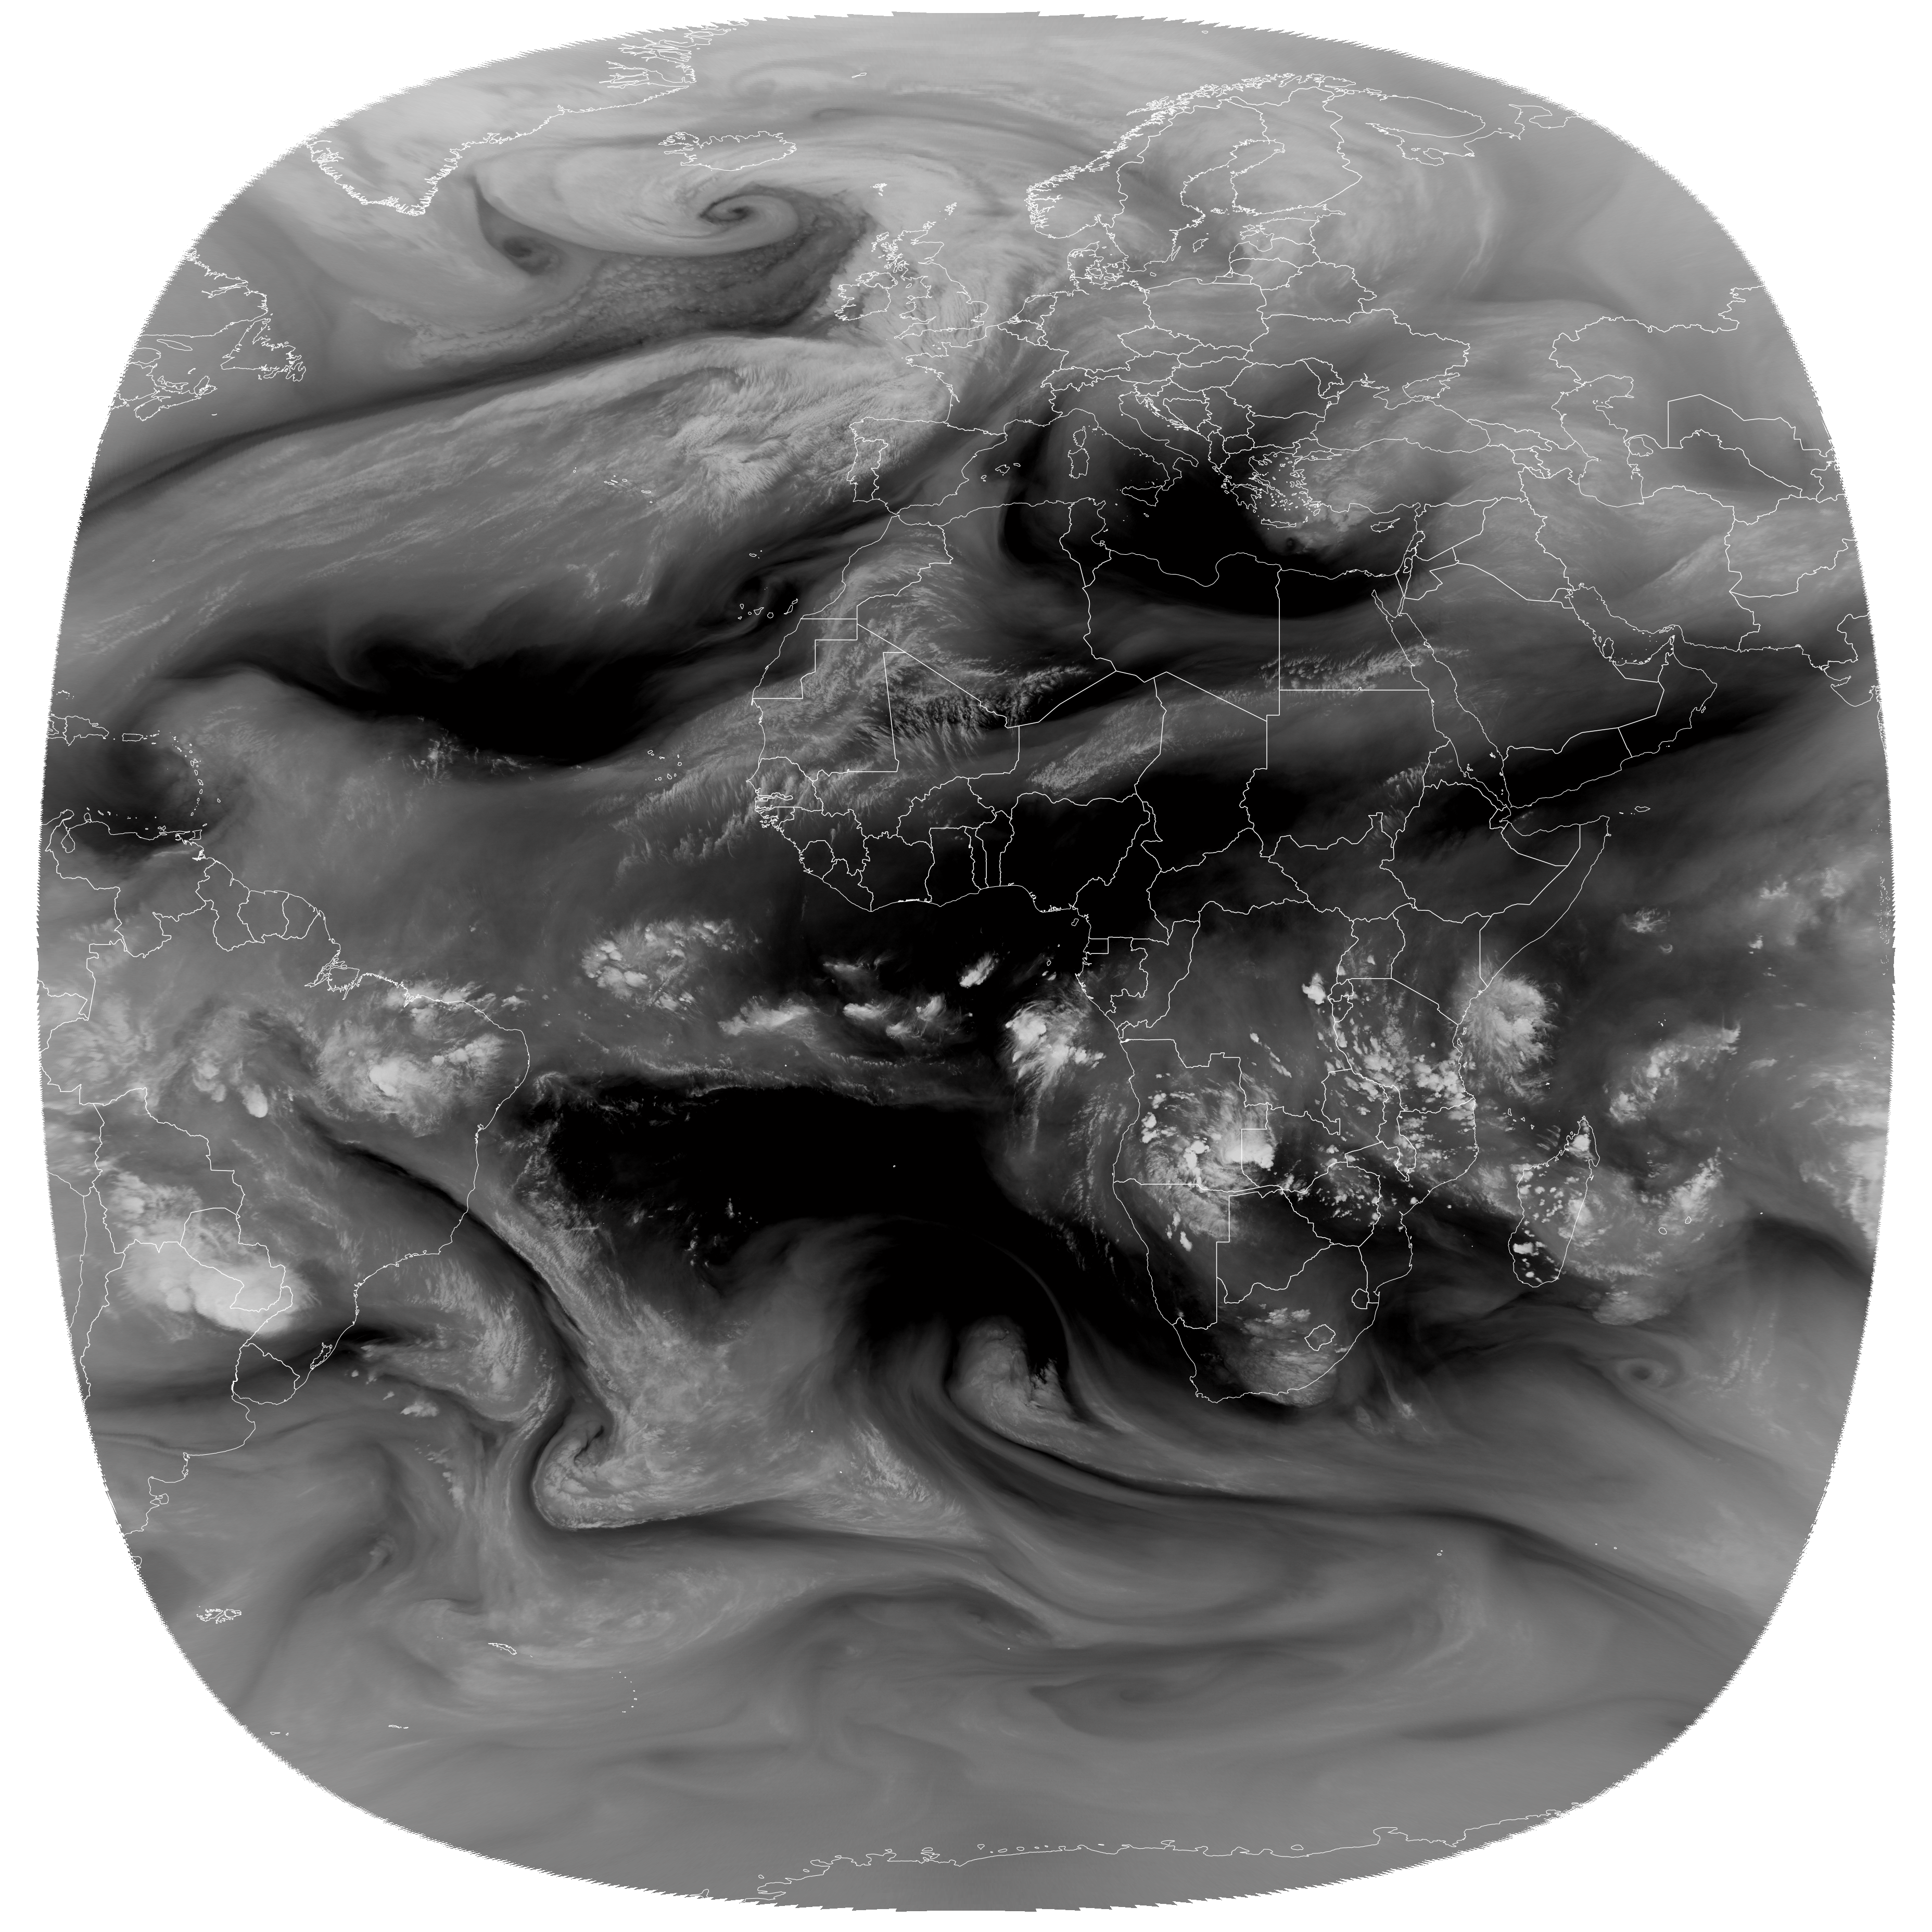
\includegraphics[width=\textwidth]{Chapter2_Theory/images/sat_channels/meteosat-msg_wv062_overlay-ne_10m_coastline_overlay-ne_10m_admin_0_boundary_lines_land.png}
            \caption[Channel WV 6.2]%
            {{\small Channel WV 6.2}}    
            \label{fig:WV_6.2}
        \end{subfigure}
        \hfill
        \begin{subfigure}[b]{0.475\textwidth}  
            \centering 
            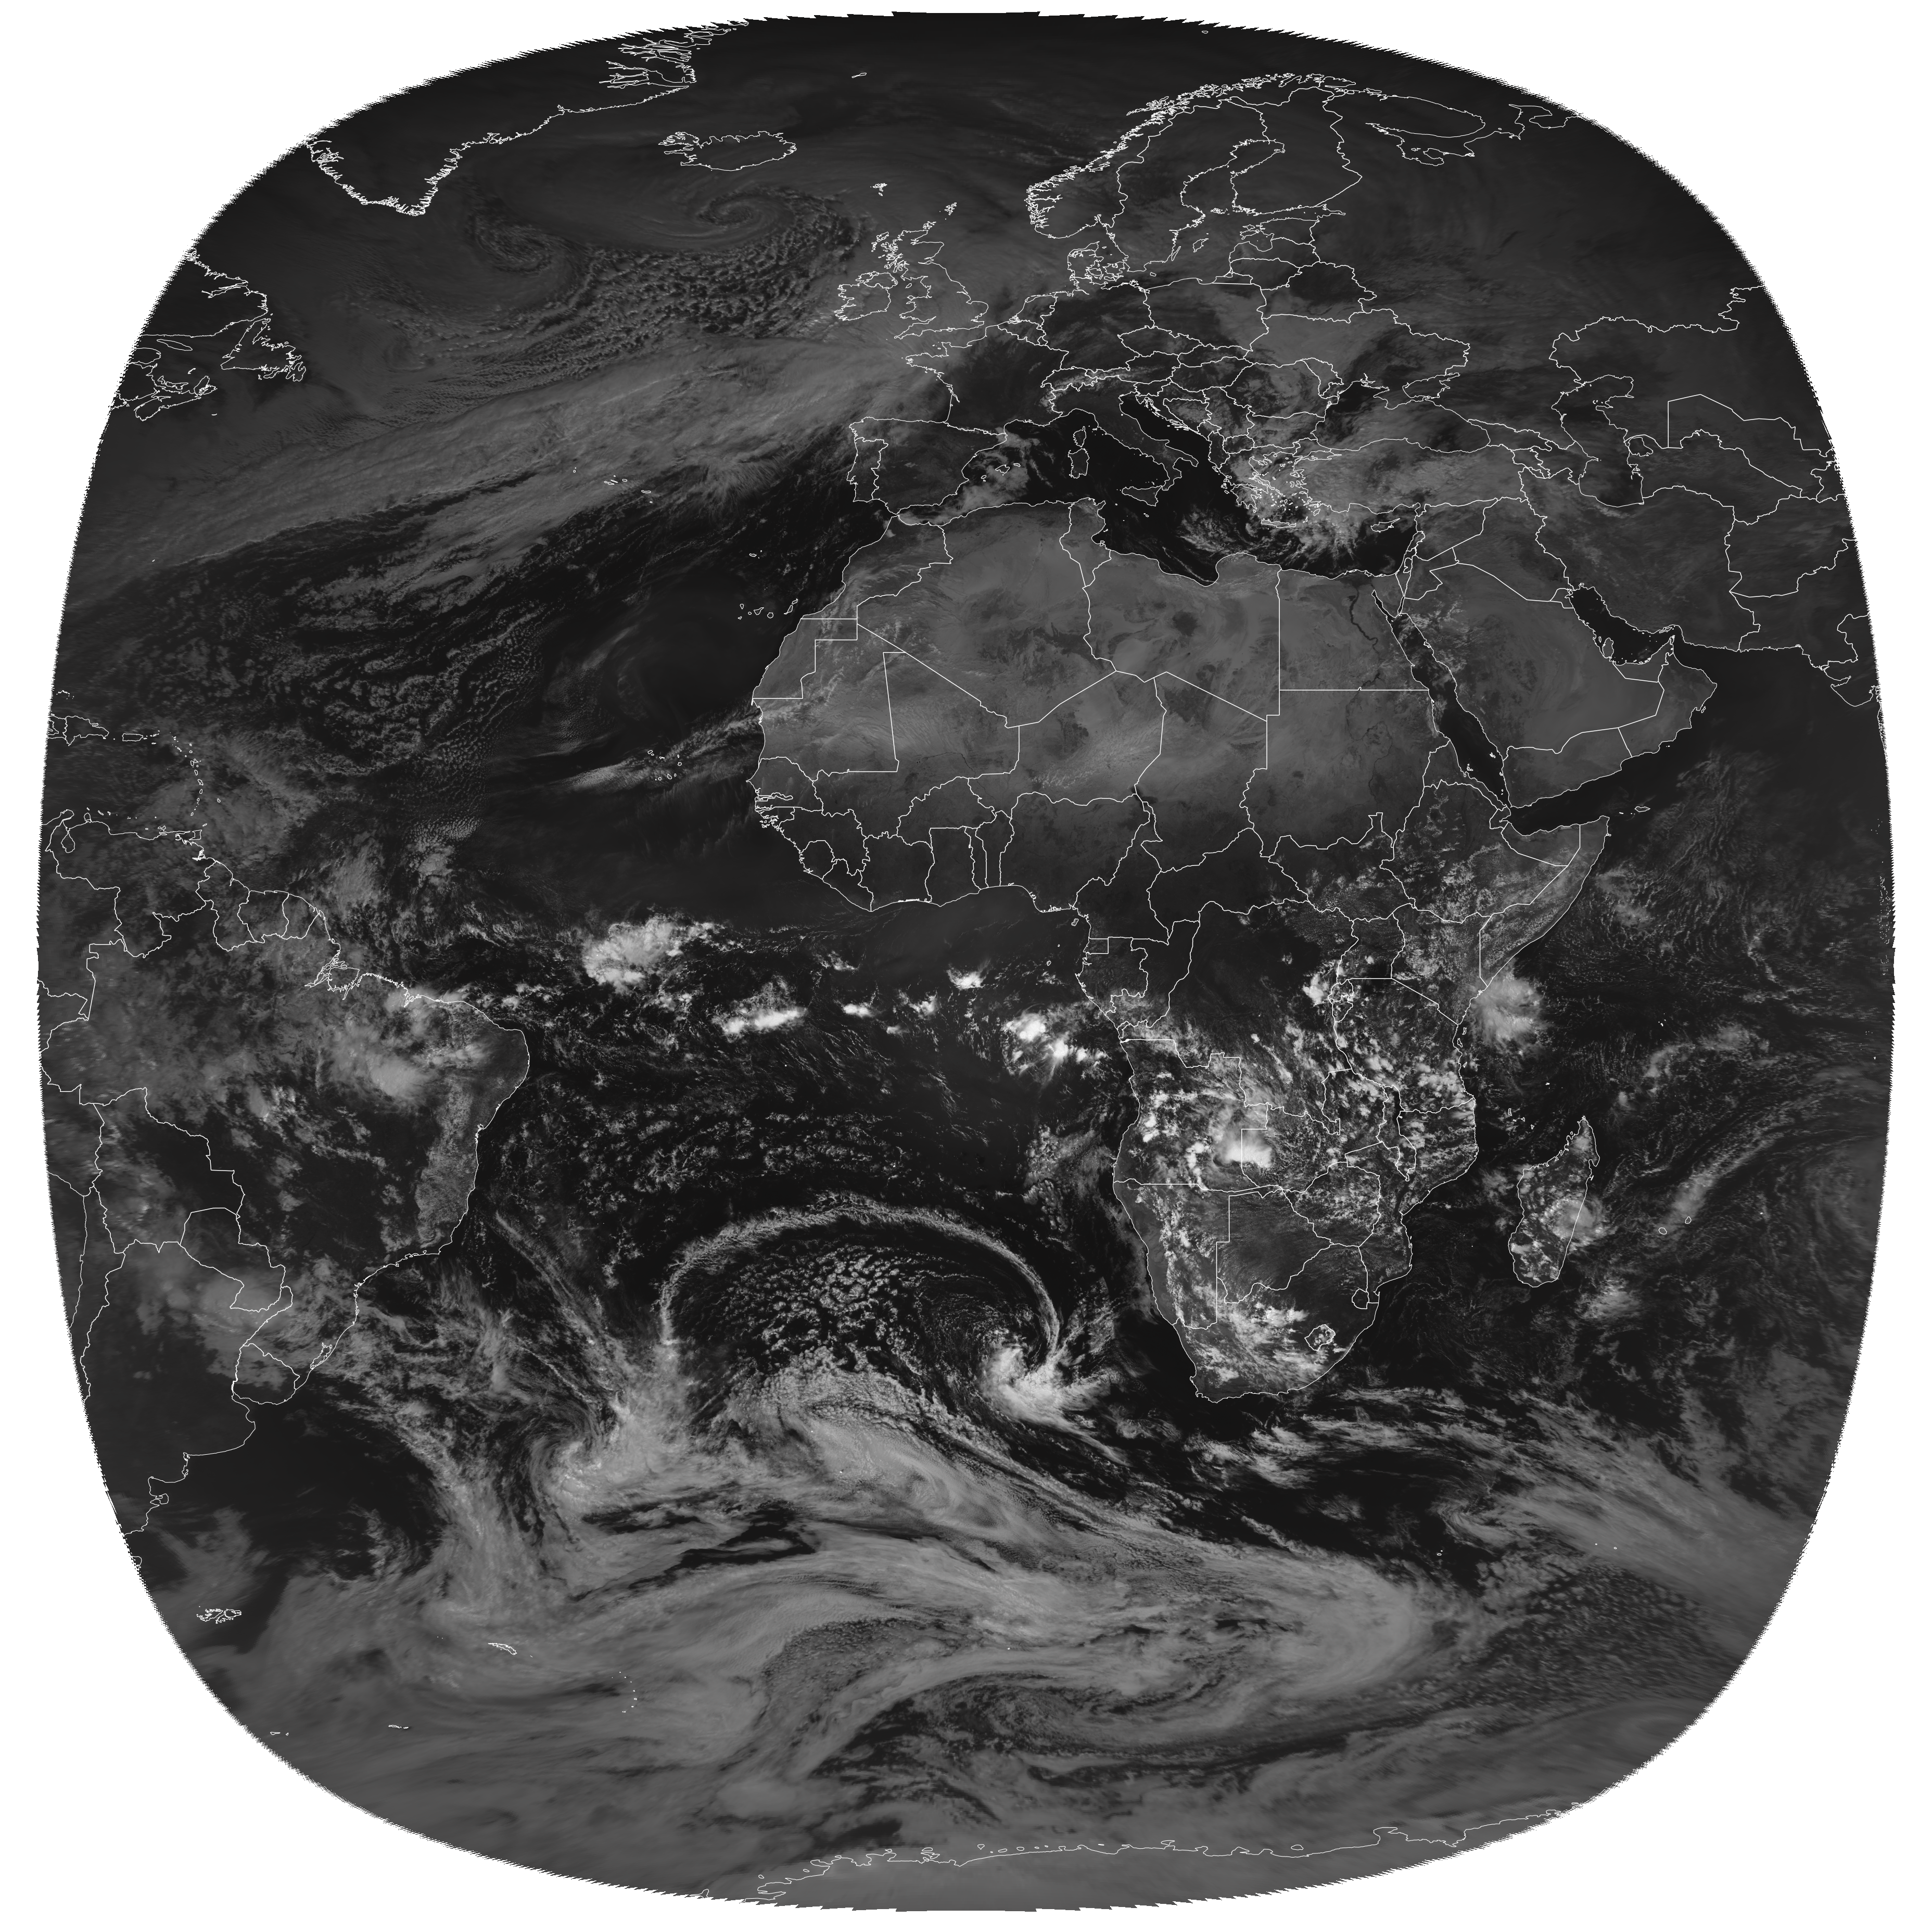
\includegraphics[width=\textwidth]{Chapter2_Theory/images/sat_channels/meteosat-msg_vis006_overlay-ne_10m_coastline_overlay-ne_10m_admin_0_boundary_lines_land.png}
            \caption[]%
            {{\small VIS 0.6}}    
            \label{fig:VIS_0.6}
        \end{subfigure}
        \vskip\baselineskip
        \begin{subfigure}[b]{0.475\textwidth}   
            \centering 
            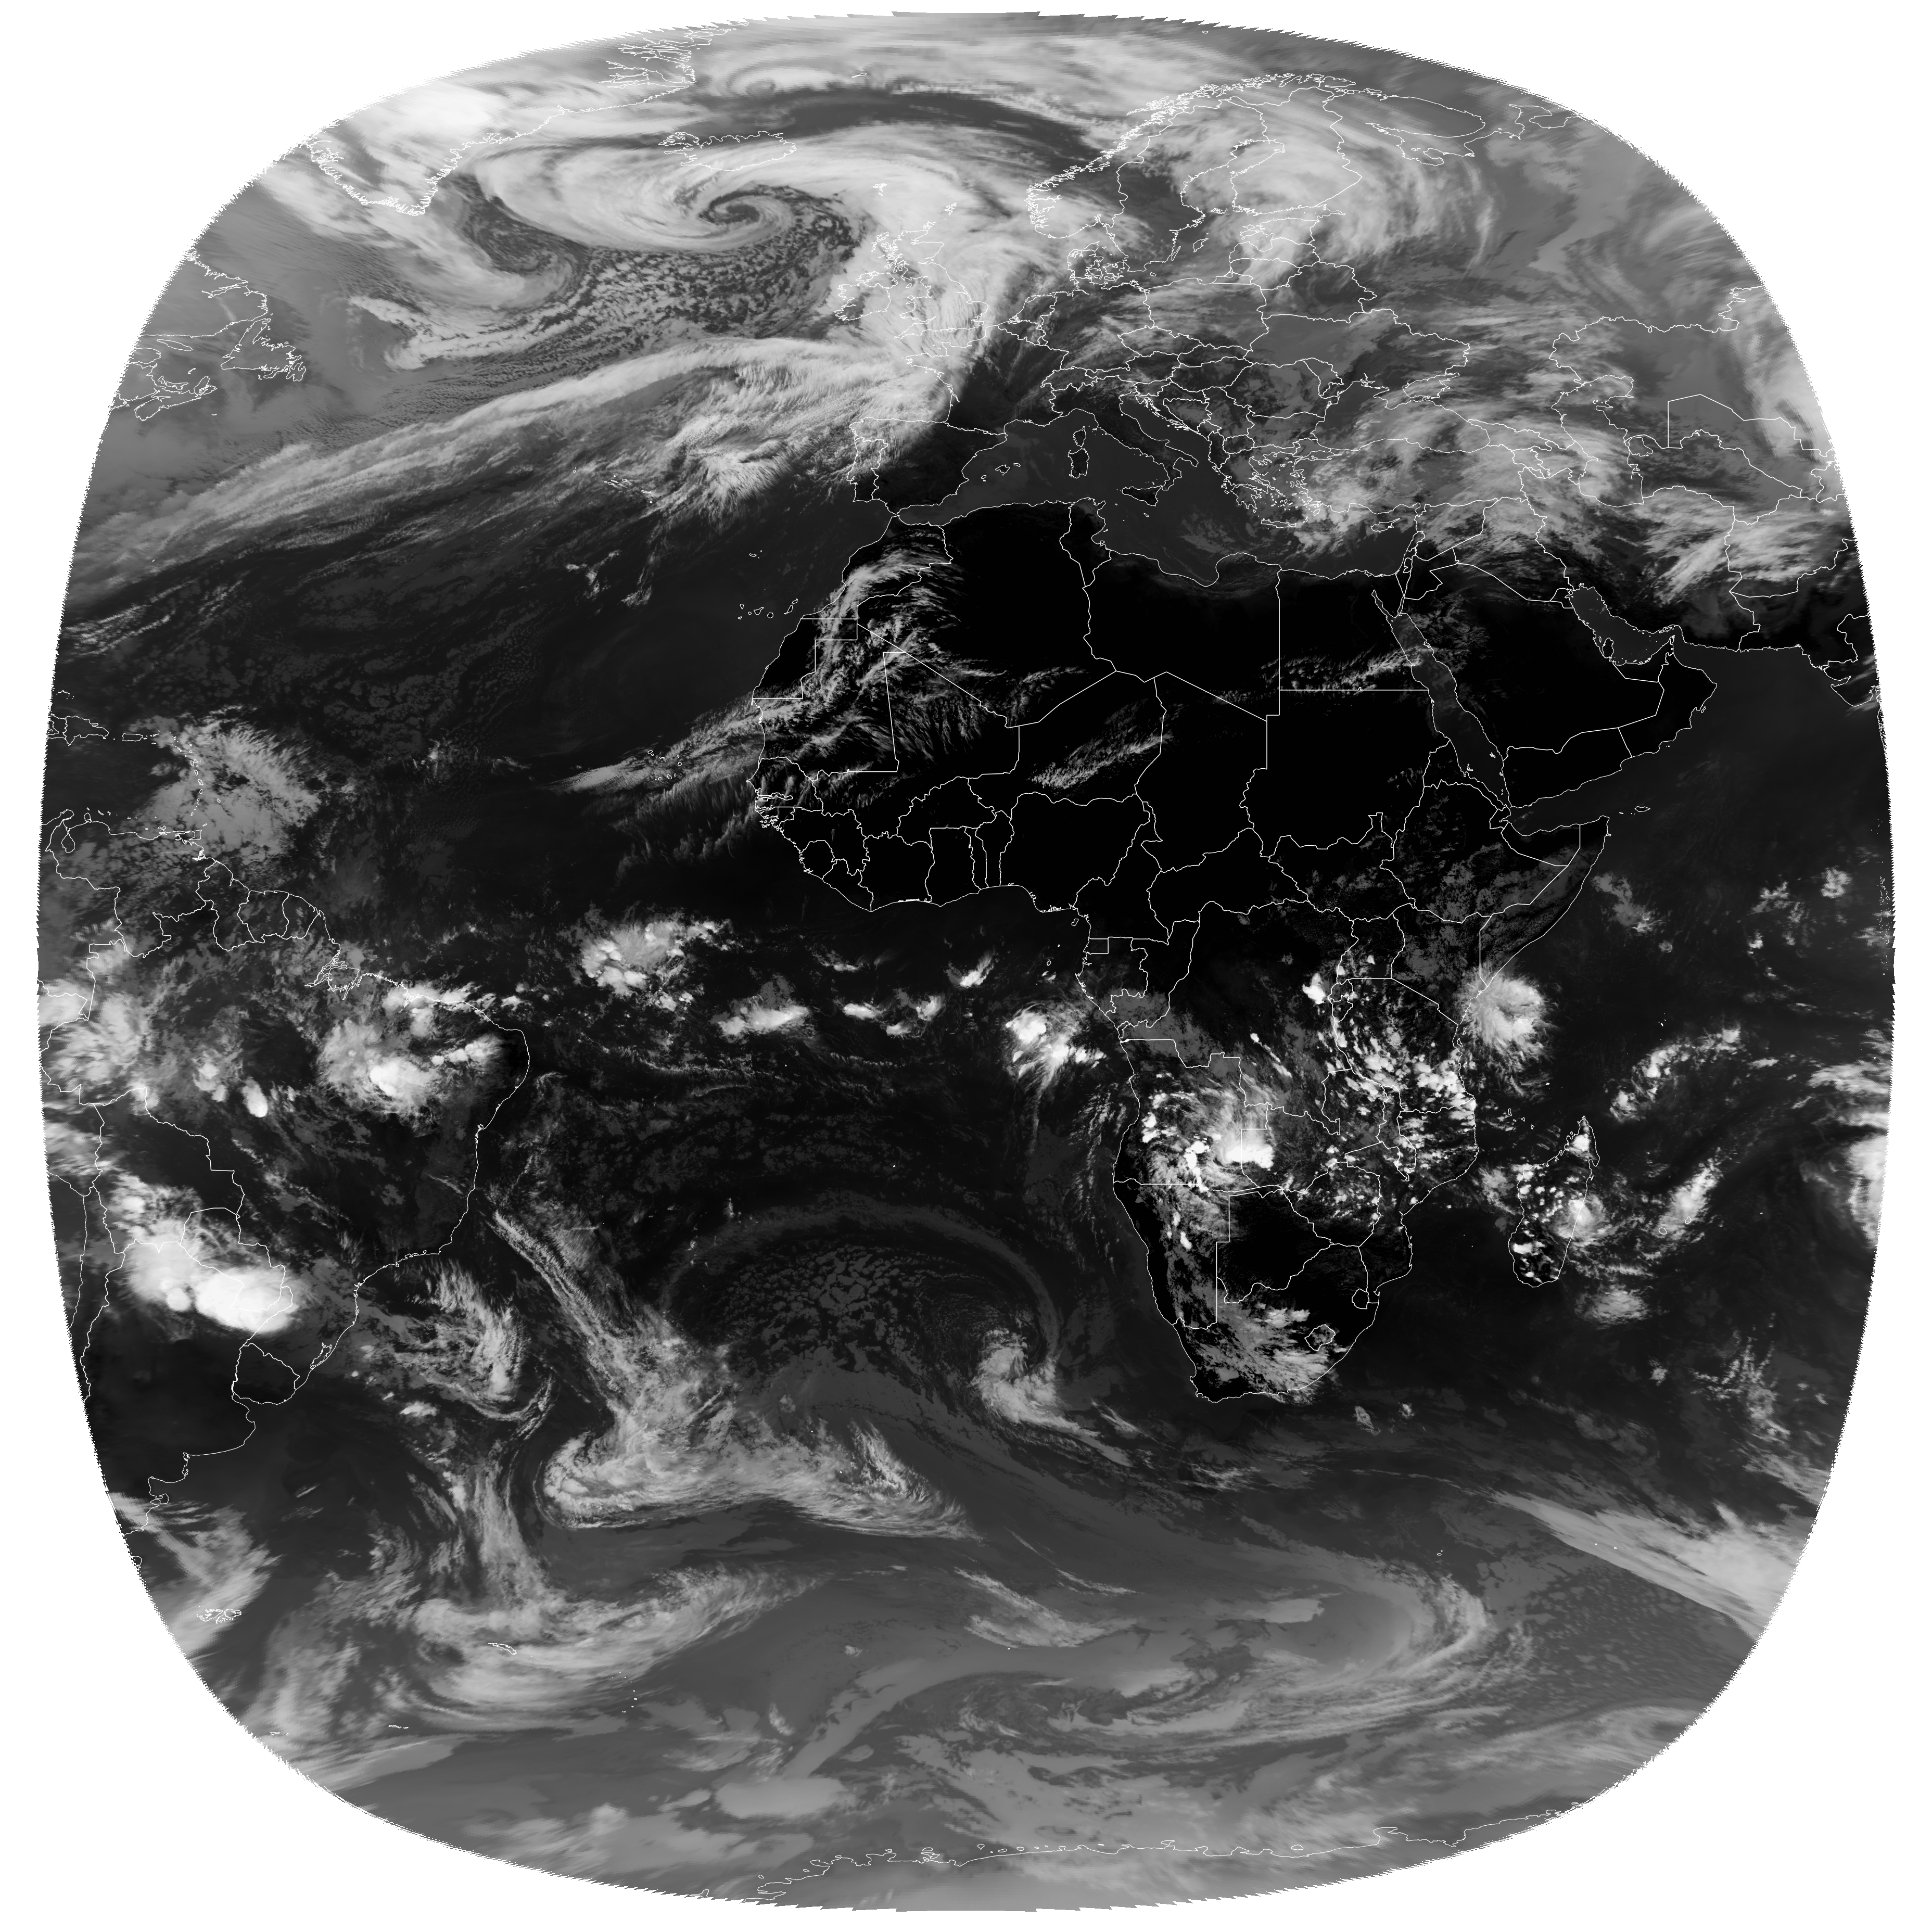
\includegraphics[width=\textwidth]{Chapter2_Theory/images/sat_channels/meteosat-msg_ir108_overlay-ne_10m_coastline_overlay-ne_10m_admin_0_boundary_lines_land.png}
            \caption[something]%
            {{\small IR 10.8}}    
            \label{fig:IR_10.8}
        \end{subfigure}
        \quad
        \begin{subfigure}[b]{0.475\textwidth}   
            \centering 
            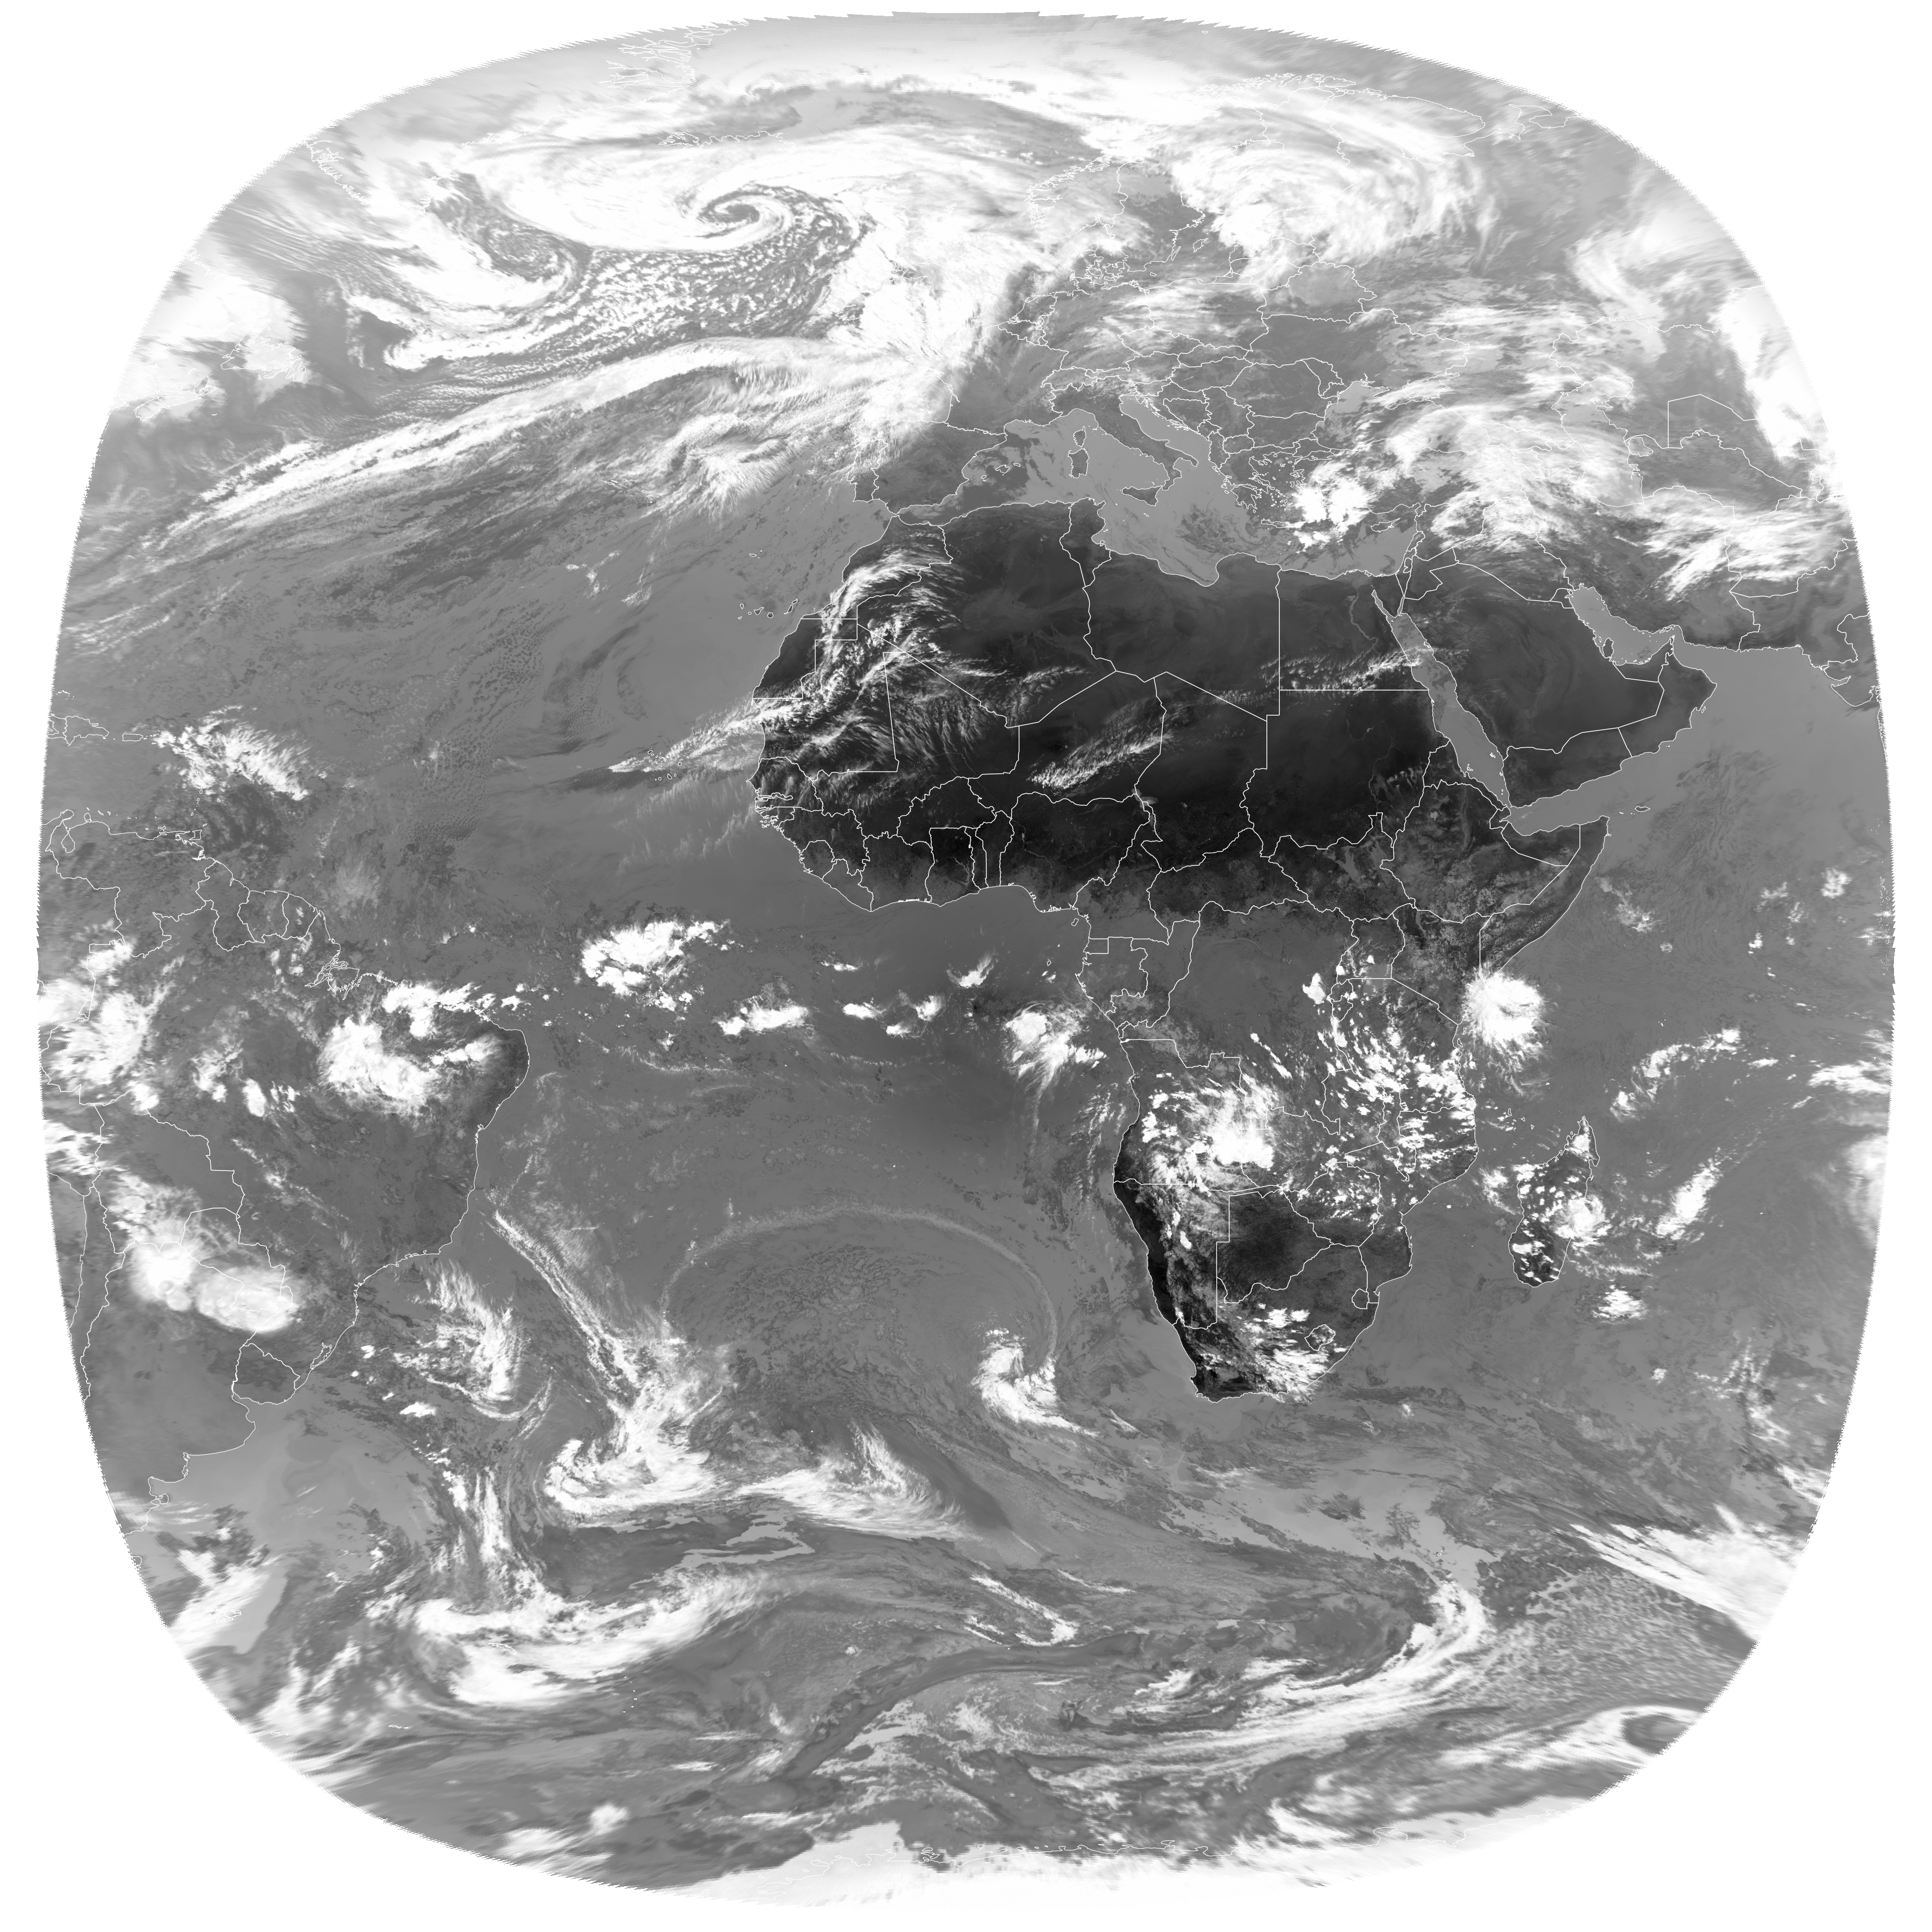
\includegraphics[width=\textwidth]{Chapter2_Theory/images/sat_channels/meteosat-msg_ir039_overlay-ne_10m_coastline_overlay-ne_10m_admin_0_boundary_lines_land.png}
            \caption{{\small IR 3.9}}    
            \label{fig:IR_3.9}
        \end{subfigure}
        \caption{{Spectral bands from SEVIRI. February 15th 2020 at noon. It shows the lowpressure system \textit{Elsa} positioned of the west coast of Iceland. Having a record breaking low of 915hPa (\cite{nrk_lavtrykk}). 
        The images are provided by  \cite{eumetcast_image_gallery}.}
    } 
    \label{fig:SEVIRI_channels}
\end{figure*}

% Info på bildene \textbf{Rectified (level 1.5) Meteosat SEVIRI image data. The data is transmitted as High Rate transmissions in 12 spectral channels. Level 1.5 image data corresponds to the geolocated and radiometrically pre-processed image data, ready for further processing, e.g. the extraction of meteorological products. Any spacecraft specific effects have been removed, and in particular, linearisation and equalisation of the image radiometry has been performed for all SEVIRI channels. The on-board blackbody data has been processed. Both radiometric and geometric quality control information is included. Images are made available with different timeliness according to their latency: quarter-hourly images if latency is more than 3 hours and hourly images if latency is less than 3 hours (for a total of 87 images per day). To enhance the perception for areas which are on the night side of the Earth a different mapping with increased contrast is applied for IR3.9 product. The greyscale mapping is based on the EBBT which allows to map the ranges 200 K to 300 K for the night and 250 K to 330 K for the day.}
% Lastet ned 16.02.2020.

\citepaper{Karlsson2015AdvancingData} list the five key properties exploited in remote sensing of clouds using passive imagery, these will be explained drawing examples from Figure \ref{fig:SEVIRI_channels}. High radiances are displayed in white and lower in darker colours. In general anything that appears bright has a higher reflection at the \acrshort{toa} than the surface. 

(1) Clouds appear bright as opposed to ice free water surfaces and vegetated Earth's surface in \acrshort{vis} and \acrshort{nir}. The detection from VIS 0.6 is shown in Figure \ref{fig:VIS_0.6}.

(2) Clouds consisting of liquid droplets reflect strongly in \acrfull{swir} and \acrfull{mwir}. The signal from MIR 3.9 is displayed in Figure \ref{fig:MIR_3.9}. Here the Earth's surface, including snow and ice, appear dark. Clouds are not perfectly emmiting black bodies and this allows for detection of low level clouds at night.

(3) Clouds are typically colder than the Earth's surface. Therefore they appear bright in IR channels, when displayed in reverse i.e. with low radiences shown as bright.

(4) Cirrus cloud are optically thin, but can be detected using split window channels (\acrshort{ir}10.8 and \acrshort{ir}12.0) differences (see Figure \ref{fig:IR_10.8}). 

(5) The last property not shown in this figure is the fact that broken clouds typically give rise to scattered patterns or texture in images with otherwise homogeneous, ice-free ocean for instance. 

Figure \ref{fig:WV_6.2} also show the signal detected from WV 6.2, water  vapour have a absorbtion band at these wavelength useull for detected water vapour. 

To summarise, the success of a screening is dependent on the illumination, the state of the surface and atmosphere. And it has proven most difficult over bright surfaces like snow and dessert (\cite{Karlsson2015AdvancingData}). 

Improved technologies allow for measuring new variables, one example of such advances is the use of active sensors. Active sensors provide a more refined image of vertical profiles and allows for the detection of cloud phase. Despite the limitations of passive sensors they provide useful historical information and in some cases higher spatial and temporal resolutions. One attempt to relate passive measurements with active measurement under the same meteorological conditions is the \textit{Afternoon constellation, A-Train} launched as a cooperation between several space agencies; \acrfull{nasa}, \acrlong{jaxa} and the french \acrfull{cnes}. This has provided a useful link between the different types of measurements (\cite{Stephens2018CloudsatSystem}). 

The number of spectral bands and footprint size (pixel resolution) determine the practical application of a particular satellite retrieval. Differences in swath width determine the frequency at a given position, determining the temporal resolution. The viewing angle affects the optical properties of the medium, and also its apparent position. \textit{Parallax} describes the apparent shift in position of a object, caused by moving the observer along an axis. This is a known issue in remote sensing. Positions of satellites are changed. Moving the observer (satellite) changes the apparent position of the measurement. 
High viewing angles may cause similar issues, in detection of high clouds. This factor is negligible when detecting low clouds (\cite{Joro2010ComparisonFinland}). 

Differences in sensitivity and retrieval algorithms contribute to a large spread in global mean cloud amount among different cloud products. This also explains the difficulties involved in using one cloud dataset to evaluate another one. In their assessment of global cloud datasets \citepaper{Stubenrauch2013AssessmentPanel} compared the global mean cloud cover of six datasets (ISCCP, PATMOS-x, MODIS-ST, MODIS-CE, AIR-LMD and TOVS Path-B). In this process they eliminating MISR and ATSR-GRAPE because of different observation times (see Table 3 in \citepaper{Stubenrauch2013AssessmentPanel} ) and two outlier datasets, HIRS-NOAA and POLDER. Their results show that the difference among the six datasets is of order 0.08. In contrast, local differences could be up to 0.4 (\cite{Stubenrauch2013AssessmentPanel}). 

%%%%%%%%%%%%%%% NOTAT I TILFELLE JEG TENKTE JEG BURDE INKLUDERT FLERE DETALJER OM FLERE DATASET.
%Cloud-Aerosol Lidar and Infrared Pathfinder Satellite Observations, CALISO is much used in other research because it gives a vertically resolved cloud (3D observations). This additional spatial information is provided on the expense of frequency and uncertainty. \textit{Reason why calipso is ruled out as a candidate. large uncertainty Stubenau} MODIS has low spatial resolution but high temporal resolution, one to two days. National Oceanic and Atmospheric Administration, NOAA \textbf{ something}. Most polar orbiting satellites have a resolution at best daily. \textbf{kilde (shubenau)} \textbf{Does the other one give ferdig produkter av skyfraksjoner og eller er mye lettere og regridde??} The number of channels (higher for other than METEOSAT). The more channels you have the more accurate cloud detection algorihms you can use. Most of the uncertainty in satellite retrivals are attributed to the presence of clouds.  

\subsection{METeosat Second Generation, MSG} \label{sec:meteosat}
The \acrfull{msg} was established as a corporation between \acrfull{esa} and \acrfull{eumetsat}. \acrshort{esa} was in charge of developing the prototype of MSG-1. \acrshort{eumetsat} is responsible for maintaining the user requirements, launch procedures, developing ground segments, ensuring overall system consistency and day to day operations. 

The primary function of \acrshort{msg} is to provide continuous observations of the Earth's full disk. Near-constant sampling frequency and a geostationary orbit allows for observing weather phenomena occurring on short timescales. Located at $0^o$ \acrshort{msg} provides a varying spatial resolution, unlike the polar orbiting satellites. The resolution gets coarser with increasing off-nadir viewing angle (\cite{Stubenrauch2013AssessmentPanel}). There are efforts invested in extending the MSG dataset with the \acrfull{mfg}, in order to make use of the time series all the way back to 1980 (\cite{Bojanowski2018PerformanceGenerations}). This requires new cloud detection algorithms since they only have three common channels and only two of them are useful for detecting clouds (\cite{Stockli2019CloudApplications}). 
\begin{table}[ht]
    \centering
    \setlength\extrarowheight{-7pt}
    \begin{tabular}{c|c|c}
        Spectral band & Central wavelength $\left( \mu m  \right)$ & Remark \newline 
        (main gaseous observer of window) \\ \hline
        VIS 0.6 & 0.635 & clouds (window)    \\
        VIS 0.8 & 0.81  & clouds (window)     \\
        NIR 1.6 & 1.64  & clouds (window)    \\
        IR 3.9 & 3.92  & clouds  (window)     \\
        WV 6.2 & 6.25 & \acrlong{wv}  \\
        WV 7.3 & 7.35 & \acrlong{wv}  \\ 
        IR 8.7 & 8.7 &   clouds  (window)       \\
        IR 9.7 & 9.66 & Ozone        \\
        IR 10.8 & 10.8 & Cirrus Clouds (window)  \\
        IR 12.0 & 12 & Cirrus Clouds (window) \\
        IR 13.4 & 13.4 & Carbon Dioxide  \\
        HRV & 0.75 & \acrlong{wv}/ window 
    \end{tabular}
    \caption{Summary of spectral bands, central wavelength and their respective retrieval abilities (\cite{Schmetz_meteosat_intro}). \textbf{Double check remark column wft is a window}}
    \label{tab:msg_spectral_bands}
\end{table}

On board the \acrshort{msg} is the \acrfull{seviri} imaging radiometer. It has 12 spectral channels. The scan is done south to north, east to west. The wavelengths of the discrete channels are chosen based on heritage from other sensors. \arcshort{seviri} has one broadband visible channel, three solar channels (0.6, 0.8 and 1.6 $\mu m$) and 8 thermal infrared channels (3.9, 6.2, 7.3, 8.7, 9.7, 10.8, 12.0 and 13.4 $\mu m$) (\cite{Taravat2015MultilayerMasking}). Table \ref{tab:msg_spectral_bands}
 gives a summary of which properties is retrive by the different channels. 
This is of great advantage since much of the community already knows how to use the \acrshort{seviri} radiance observations. The channels have been chosen based on their ability to detect clouds, water vapour and ozone. More information about what the different channels detect is available in the paper \textit{An introduction to METeosat second generation (MSG)} published in \acrshort{bams} by \citepaper{Schmetz_meteosat_intro}.

Prior to the launch of the METeosat researchers discussed the temporal frequency suitable for observing weather phenomena. The METeosat first generation had a temporal resolution of 30min (\cite{Stockli2019CloudApplications}). For the second generation, 15min intervals were chosen to best cope with the short lifetime and rapid deformation of clouds. It was also suggested that a temporal frequency of 1 to 10min is necessary for tracking cumulus type clouds (\cite{Schmetz_meteosat_intro}). % 987 
This is in agreement with the Table 1.3 in \citeauthor{lohmann2016} (\citeyear{lohmann2016}, p. 19) stating the lifetimes of different types of clouds.

A \textit{ring} of geostationary satellites located at equator together provide global coverage (excluding polar regions). The altitude of the satellite determines its forward velocity. To achieve a geosynchronous orbit, a satellite needs to maintain a height of $\sim 36 000km$ (\cite{Bley2013ASEVIRI}). This height lead to a coarser spatial resolution than other satellite products retrived from other orbits. 

The first METeosat Second Generation (MSG-1) was launched 28 August 2002, and became operational 29 January 2004 when it was renamed METeosat-8. As a measure to reduce gaps, the \acrshort{msg} system provides a two-satellite system, one operational and one standby. The standby satellite scans when the operational satellite experiences technical failures. 
The operational satellite at nadir points at $0^o$ latitude. A full disk is $3712\times 3712$ pixels, and is sampled in cycles of 15min. This also include the on-board processing (\cite{Schmetz_meteosat_intro}).

\begin{figure}[h]
    \centering
    \includegraphics[scale=0.11]{Chapter2_Theory/images/MET10_RGBNatColourEnhncd_FullResolution_20191123120000.jpg}
    \caption{The view of Earth by \acrshort{seviri} on \acrshort{msg}, in naturally enhanced colours. This snapshot is dated noon 23rd of November 2019. By studying this image it becomes clear that clouds are influenced by circulation  (\cite{eumetcast_image_gallery}).}
    \label{fig:sat_view}
\end{figure}
The operational cloud detection algorithm is carried out pixel by pixel. Post processing involves re-classifying isolated pixels. There is a lot of effort invested in new detection algorithms including spatial structures. One of the methods that show potential here is deep learning (\cite{Dronner2018FastNetworks}, \cite{jeppesen_deep_cloud_masking}).

\subsection{EUMETSAT Cloud Mask} \label{sec:EUMETSAT_cloud_mask}
The \acrshort{eumetsat} cloud mask (CLM) consist of four classes, described in Table \ref{tab:classes_clm}.
\begin{table}[h]
    \centering
    \setlength\extrarowheight{-7pt}
    \begin{tabular}{c|c}
        Class & Description \\ \hline
        0 & Clear sky over ocean \\
        1 & Clear sky over land \\
        2 & Cloudy \\
        3 & No data/ outer space        
    \end{tabular}
    \caption{Description of classes in EUMETSAT Cloud Mask product.}
    \label{tab:classes_clm}
\end{table}
These classes are derived from almost all channels except the broadband \acrshort{hrv} and isolated pixels are reclassified (\cite{Tavarat10_Derrien}). The cloud mask is distributed in \acrfull{grib},  without coordinates and \acrfull{netcdf}, processed with coordinates and reshaped into the standard rotation, as displayed i Figure \ref{fig:sat_view} The data is available via Earth Observation Portal on \acrshort{eumetsat}'s web pages. 

